\section{Introduction to Extended Reality}
\label{sec:background-intro}

Extended Reality (XR) is an umbrella term encompassing all the possible combinations of real and virtual environments included in the spectrum of the “Reality-Virtuality Continuum” (see \autoref{fig:virtuality-continuum}), introduced by Paul Milgram and Fumio Kishino in 1994 \cite{milgram_taxonomy_1994}.

\begin{figure}[h]
	\centering
	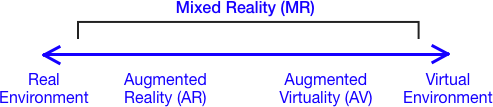
\includegraphics[width=7.5cm]{virtuality-continuum.png}
	\caption{Milgram and Kishino's \textit{Reality-Virtuality Continuum}}
	\label{fig:virtuality-continuum}
\end{figure}
In their work, the authors considered the real environment and virtual environment (VE) as two sides belonging to the same continuum, instead of two words in antitheses. Between them there are other concepts with a variable quantity of real and VE such as Augmented Reality (AR), that allows users to see the real world with virtual objects superimposed upon it, and Augmented Virtuality, in which objects from the physical world augment the virtual environment. Eventually, Mixed Reality (MR) has the peculiarity of mixing these two concepts, in which physical and virtual objects co-exist and interact in real time with the user.

Some more emphasis on AR is put by Ronald Azuma \cite{azuma_survey_1997}, where the author defined three academic criteria for AR: it \textit{“combines the real and virtual”}, it is \textit{“interactive in real time”} and it is \textit{“registered in three dimensions”}. Later, Azuma et al.~\cite{azuma_advances_2001}, added that AR's objective is to \textit{“enhance the user’s perception of and interaction with the real world”}.

The “X” of XR represents a variable for any of these existing combinations. We have Augmented Reality (X=A, AR), Mixed Reality (X=M, MR) and Virtual Reality (X=V, VR). XR not only covers these environments but, as Honkanen \cite{honkanen_enhancing_2018} states, it is also the common term representing their immersive technologies and \textit{“human-device interaction aspects”}. Suh and Prophet \cite{suh_prophet_2018}, in their literature review on immersive technologies, describe XR as a means through which users' reality is extended as they feel placed within a simulation in a way that real and simulated environments become indistinguishable \cite{kwok_covid-19_2020}.

A technical background of AR and VR is given by Egger et al.~\cite{egger_augmented_2020}. Augmented objects in AR are seen through a visor that consists of a device with a camera that captures frames from the external world and a display that shows the virtual components superimposed over the real view. The frames captured by the camera, before being shown in their final presentation, are processed by a software able to recognize the real environment and track features like the position, the elements in the scene and the 3D coordinates of the camera.
The authors differentiate marker-less and marker-based tracking: the latter uses image recognition systems to identify tags on the objects and track them; the former can use GPS, accelerometer, ultrasounds, opto-electronic sensors or inertial sensors.
In order to implement an AR system three different types of displays have been identified:
\begin{enumerate}
	\item Head-mounted displays (HMDs), or “see-through AR glasses”, are a wearable device that work as normal glasses and contemporaneously have a small projector on the lenses to augment the real world with additional contents. The real environment is captured by the users by freely moving around it.
	\item Handheld devices equipped with all the components needed to record the real world and track its objects, e.g. camera, accelerometer and GPS. Most smartphones are equipped with these built-in instruments making AR widely used on mobile devices.
	\item Other forms of displays that do not belong to the previous two categories for simplicity indicated as Mobile AR (MAR). An example of these displays are the AR mirrors often placed in open spaces that \textit{“do not require users to depend on any kind of device or application to experience AR”}.
\end{enumerate} 
VR, on the other hand, renders a totally VE that, according to Guttentag \cite{guttentag_virtual_2020}, can be navigated and interacted with by the users, of which one or more of their five senses are simulated in real-time. The author's study also defines two characteristics of VR: the ability to provide a physical immersion and a physical presence, making participants behave as in a real-life situation.
The VE, as explained by Egger et al., can represent either a computer-generated world, a 360° real-captured video or image.

Beck et al.~\cite{beck_2019_virtual} classify VR systems (VRs) distinguishing between non-, semi- and fully immersive VRs. The first term classifies desktop solutions allowing to navigate 360° videos and images in a classical PC interaction through a mouse or keyboard, and they are the simplest and most used form of VR, in platforms like YouTube and Facebook 360° Video. Semi-immersive systems have been used in the past years by projecting screens onto the walls and floor of a room, complementing the setting with spatial sounds for a multi-user experience.
In the end, fully immersive VRs require users to wear a HMD that supports head tracking and other interactions through, usually, controllers or wearable devices, with the resulting feeling of a complete isolation from the physical environment.

Jung and Jeong \cite{jung_classification_2020} provide a further classification of VR devices according to the physical connectivity, tracking system and user behavior. The PC-tethered VR, Console-tethered VR, Standalone VR and Smartphone VR constitute the four categories to classify a VR device on its physical connectivity, respectively: a VR headset connected to a desktop computer and a video game console that render the VE, a VR headset unthetered from any external device and a VR system made using a smartphone to render the graphics and a headset with lenses to simulate a VR device. In terms of tracking systems two technologies are used to track user's motion, the head tracking and position tracking: the latter uses internal sensors of the headset (e.g. gyroscope, accelerometer and magnetometer), the former can be again divided into inside-out position tracking, using a camera on the headset to determine the movement, and outside-in position tracking that relies on external devices.
For what concerns user behavior categorization, VRs are divided into stationary VR, desktop-scale VR, room-scale VR and mobility VR. A VR device that does not have a position tracking feature can only be used in a stationary way, belonging to the stationary VR category; the desktop-scale VR and room-scale VR are opposites and refer to, respectively, systems with a restricted position tracking coverage and systems with a wider one. Eventually, a mobility VR device does not have space constraint and can, therefore, be used without spatial restrictions given its untethered nature and stand-alone position tracking component.